\documentclass[conference]{IEEEtran}
%future work: local patch operator
%complexity
\usepackage{bigstrut}
\usepackage{balance}
\usepackage{subfig}
\usepackage{wrapfig}
\usepackage{amsmath}
\usepackage{url}
\usepackage{pifont}
\usepackage{mdframed}
\pagenumbering{gobble}
\usepackage{lettrine}
%\usepackage{times}
\usepackage{rotating}
\usepackage{booktabs}
%\usepackage{balance} 
\usepackage{color, colortbl}
\usepackage{graphicx}
\usepackage{algorithmicx}
\usepackage[running]{lineno}
\usepackage{times}
\usepackage{fancyhdr,graphicx,amsmath,amssymb}
\usepackage[ruled,vlined]{algorithm2e}
\include{pythonlisting}
\usepackage{program}
\usepackage{cite}
\usepackage{alltt}
\usepackage{balance}
\newcommand{\eq}[1]{Equation~\ref{eq:#1}}
\newcommand{\bi}{\begin{itemize}}
	\newcommand{\ei}{\end{itemize}}
\newcommand{\be}{\begin{enumerate}}
	\newcommand{\ee}{\end{enumerate}}
\newcommand{\tion}[1]{\textsection\ref{sec:#1}}
\newcommand{\fig}[1]{Figure~\ref{fig:#1}}
\definecolor{lightgray}{gray}{0.975}
\usepackage{fancyvrb}
\usepackage{stfloats}
\usepackage{multirow}
\usepackage{listings}
\usepackage{amsmath}  
\DeclareMathOperator*{\argmin}{arg\,min} 
\DeclareMathOperator*{\argmax}{arg\,max} 
%\usepackage[usenames]{xcolor}
\bibliographystyle{unsrt}



\usepackage{color}
\newcommand{\colorrule}[1]{\begingroup\color{#1}\hrule\endgroup}

\definecolor{darkgreen}{rgb}{0,0.3,0}

\usepackage[table]{xcolor}
\definecolor{Gray}{rgb}{0.88,1,1}
\definecolor{Gray}{gray}{0.85}
\definecolor{Blue}{RGB}{0,29,193}
\newcommand{\G}{\cellcolor{green}}
\newcommand{\Y}{\cellcolor{yellow}}
\newcommand{\tc}{\centering\arraybackslash}
\newcommand\topspace{\rule{0pt}{2.6ex}}       % Top strut
\newcommand{\stack}[3]{\vskip 1mm\shortstack{Min : #1 \\ Med : #2 \\ Max : #3}}


\definecolor{MyDarkBlue}{rgb}{0,0.08,0.45} 
\newenvironment{changed}{\par\color{MyDarkBlue}}{\par}

\newcommand{\ADD}[1]{\textcolor{MyDarkBlue}{{\bf #1}}}
\newcommand{\addit}[1]{\begin{changed}\input{#1}\end{changed}}

\usepackage{color}
\usepackage{listings}
\usepackage{setspace}

\usepackage{array}
\newcolumntype{$}{>{\global\let\currentrowstyle\relax}}
\newcolumntype{^}{>{\currentrowstyle}}
\newcommand{\rowstyle}[1]{\gdef\currentrowstyle{#1}%
  #1\ignorespaces
}

\lstnewenvironment{python}[1][]{
\lstset{
	mathescape,
	numbers=right,
	numberstyle=\scriptsize,
	stepnumber=1,
	numbersep=0.5em,
	xleftmargin=0em,
	framextopmargin=2em,
	framexbottommargin=2em,
	showspaces=false,
	showtabs=false,
	showstringspaces=false,
	tabsize=2,
	% Basic
	basicstyle=\ttfamily\scriptsize\setstretch{0.8},
	backgroundcolor=\color{Background},
	language=Python,
	% Comments
	commentstyle=\color{Comments}\slshape,
	% Strings
	stringstyle=\color{Strings},
	morecomment=[s][\color{Strings}]{"""}{"""},
	morecomment=[s][\color{Strings}]{'''}{'''},
	% keywords
	morekeywords={[1]import,from,class,def,for,while,if,is,in,elif,else,not,and,or,print,break,continue,return,True,False,None,access,as,,del,except,exec,finally,global,import,lambda,pass,print,raise,try,assert, dot, norm, zip, sorted},
	keywordstyle={[1]\color{Code}\bfseries},
	% additional keywords
	morekeywords={[3]fastmap,Slope,bPruning,clister,train,leafs,weightedFeatures,HOW, exemplar,nearestSlope,dist,displace,geometry,splitAcross2Points,leaves,How,nearest,bPruning,Stats,divide,recurse,weight1,project, furthest, split,WHERE,clusterer, getContours,envied, fWeight, nearestContour, projection, mutate, HERE, knn},
	keywordstyle={[3]\color{Keywords}\bfseries},
	morekeywords={[2]@invari},
	keywordstyle={[2]\color{Decorators}\slshape},
	emph={self},
	emphstyle={\color{self}\slshape},
	firstnumber=last
	%
}}{}


\definecolor{Gray}{gray}{0.9}
\definecolor{Gray}{gray}{0.95}
\newcommand{\kw}[1]{\textit{#1}}
\newcommand{\quart}[4]{\begin{picture}(80,6)
	{\color{black}\put(#3,3){\circle*{2.5}}\put(#1,3){\line(1,0){#2}}}\end{picture}}

% New Commands
\usepackage{etex}
\author{Rahul Krishna, George Mathew\\
	Computer Science, North Carolina State University, USA\\
	\{rkrish11, george2\}\@ncsu.edu
}
\title{Evolutionary Multi-Objective Optimization:\\ A Distributed Computing approach}
% \usepackage{etoolbox}
\makeatletter
\makeatother


\pagestyle{plain}
\begin{document}
	\maketitle
	\begin{abstract}
		Multi-objective problems are usually complex, NP-Hard, and resource intensive. Although exact methods can be used, they consume prohibitively large amounts of time and memory. An alternative approach would be to make use of meta-heuristic algorithms, which approximate the Pareto frontier in a reasonable amount of time. Even so, these meta-heuristic algorithms consume a significant amount of time. 
		
		Parallel and distributed computing used in design and implementation of these algorithms may offer significant speed-ups. In addition to this, they may be used to improve the quality, increase the robustness of the the obtained solutions, and may also allow the algorithms to be scaled to solve large problems. 
		
		We present parallel models for two multi-objective optimization problems: Diffential Evolution(DE) and Geometric Active learner(GALE).
		
	\end{abstract}
	\begin{IEEEkeywords}
		Evolutionary Algorithms, Multi Objective Optimization, Parallelization, Pareto Frontier
	\end{IEEEkeywords}
	
	\section{Introduction} 
	
	\lettrine{M}{etaheuristic} search methods such as Evolutionary Algorithms are commonly used to \textit{optimize} many real-world applications \cite{89genetic,storn97}. Optimization is the task of finding solutions which satisfy one or more specified objectives. There are two types of optimizers, a single-objective optimization involves a single objective function and a single solution, a multi-objective optimization considers several objectives simultaneously. In case of a multi-objective optimizer generates a set of alternate solutions with certain trade-offs. These are called Pareto optimal solutions. 
	
	The design of the evolutionary algorithms naturally leads to parallelization. They contain several individuals which are being improved through generations. This parallel nature is particularly useful when implementing the algorithm on distributed systems. Many real-world applications have time consuming function evaluations and therefore parallelizing the evaluations on a set of available computing resources speeds up the optimization task. In addition to this, steady advances in new technologies such as Grid Computing \cite{abramson2000nimrod} allows parallelization to be performed with relative ease. Several Parallel Evolutionary Algorithms have been studied in the literature (e.g., in \cite{alba2002parallelism,branke2004distribution,deb2003distributed}). 
	
	There are several parallel computing strategies (models) \cite{08parallel}, here we explore the three main models --- the Island model, Master-Slave model and Diffusion model. The current focus of this paper is the Island model, where the population for a given run is divided into semi-isolated subpopulations. Each subpopulation is assigned to a separate processor of the parallel computing system. The run begins with the one-time random creation of a separate population of individuals at each processor of the parallel computer system.
	
	In this project, we aim to present parallel models for two evolutionary multi-objective optimizers: (1) Differential Evolution (DE) \cite{storn97}; and (2) Geometric Active Learning (GALE) \cite{krall15}. For implementation, we use the \textit{henry2 Linux cluster} offered by NC State with message passing (OpenMPI)~\cite{openMPI04} a distributed programming environment.
	
	This report is organized as follows. The following section presents a brief background on the pertinent topics. In \textsection\ref{algos}, we discuss various strategies for parallelization. In \textsection\ref{experiments}, we provide the preliminary results. Finally, \textsection\ref{future} highlights how we plan on following up our work.
	
	\section{Methods and Materials}
	\label{algos}
	\subsection{Evolutionary Algorithms}
	An Evolutionary Optimization(EO) begins its search with a population of solutions usually created at random within a specified lower and upper bound on each variable. If bounds are not supplied in an optimization problem, suitable values can be assumed only for the initialization purpose. Thereafter, the EO procedure enters into an iterative operation of updating the current population to create a new population by the use of four main operators: selection, crossover, mutation and elite-preservation. The operation stops when one or more termination criteria are met. The two main EO we plan to study are listed below:
	
	\subsubsection{Differential Evolution (DE)} 
	
	The Differential Evolution algorithm involves maintaining a population of candidate solutions subjected to iterations of recombination, evaluation, and selection. The recombination approach involves the creation of new candidate solution components based on the weighted difference between two randomly selected population members added to a third population member. This perturbs population members relative to the spread of the broader population. In conjunction with selection, the perturbation effect self-organizes the sampling of the problem space, bounding it to known areas of interest on the Pareto frontier. \fig{de} highlights the algorithmic details of the algorithm.
	
	\begin{figure}[h]
		\begin{mdframed}
			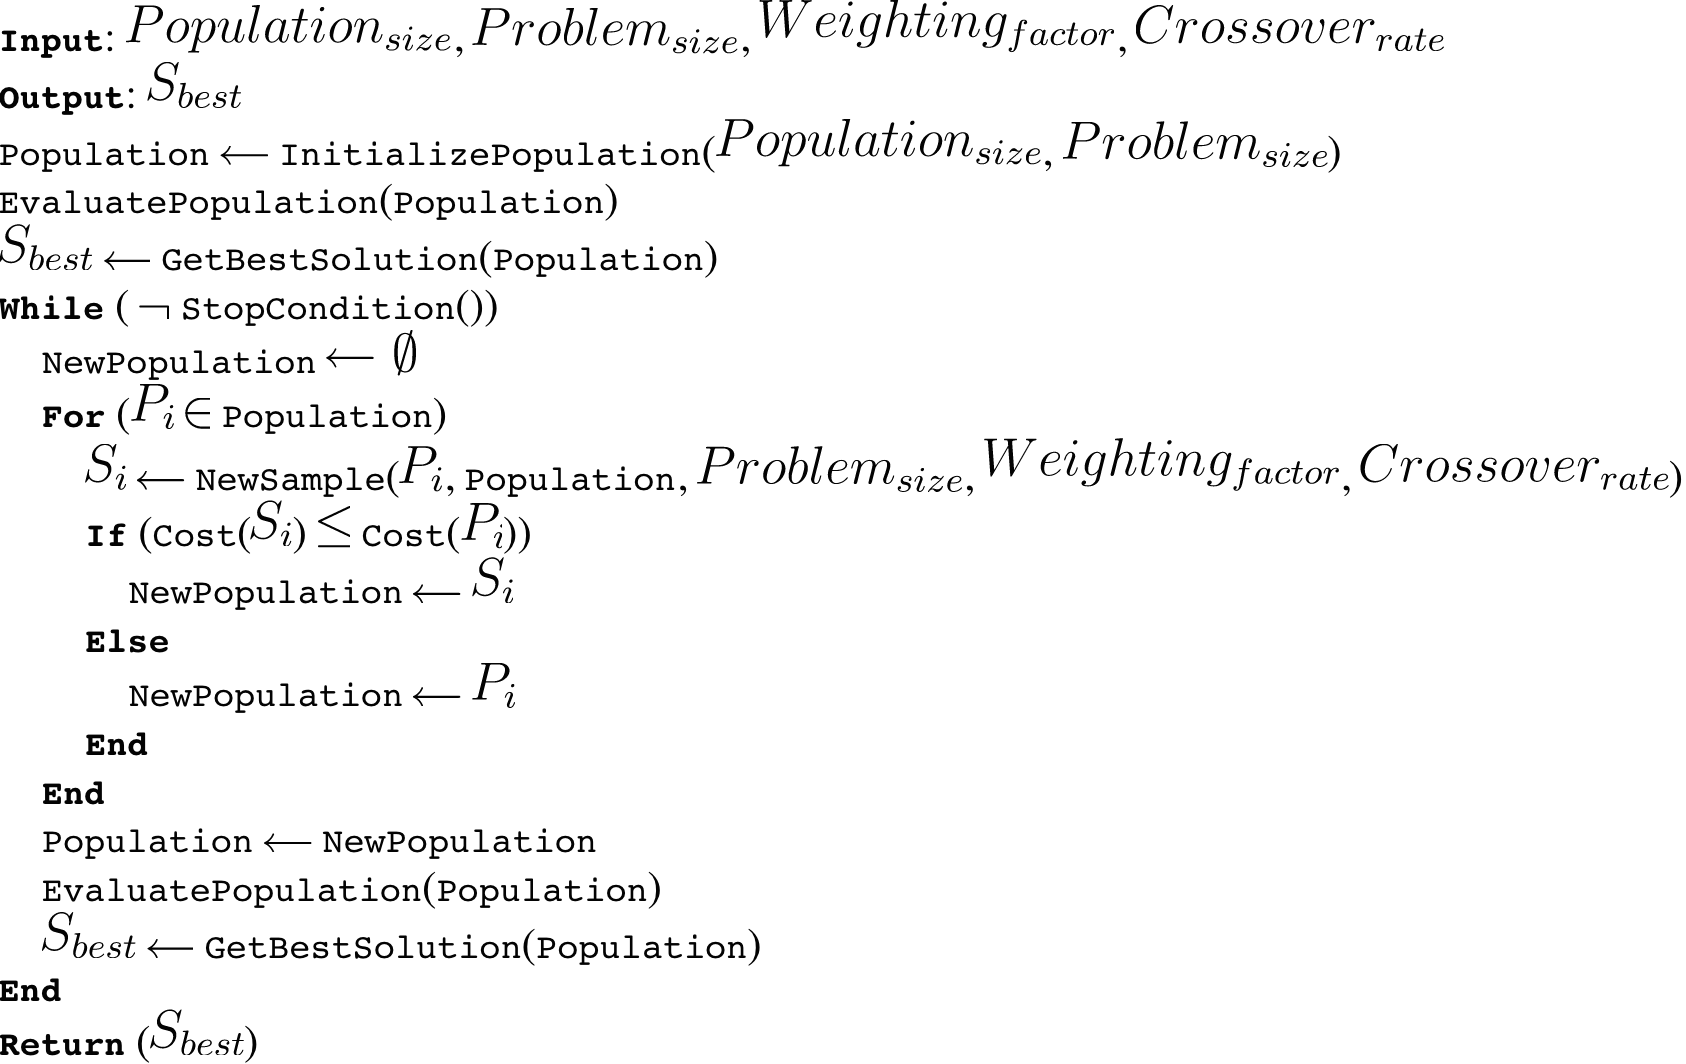
\includegraphics[width=\linewidth]{img/de.png}
		\end{mdframed}
		\caption{Algorithm: Differential Evolution}	
		\label{fig:de}
	\end{figure}
	
	
	\subsubsection{Geometric Active Learning (GALE)} 
	
	GALE is a near-linear time multi-objective optimization algorithm that builds a piecewise approximation to the surface of best solutions along the Pareto frontier. GALE uses a recursive hierarchical clustering algorithm called WHERE, which is powered by a FASTMAP \cite{faloutsos95}, to recursively reduce the dimensions to a single principal component, see \fig{where}. After clustering, the non dominated leaf is identified(i.e the leaf with the best set of solutions) and all the points within this leaf cluster is mutated along the principal component to generate a subset of the population for the next generation. The rest of the population is randomly generated over the decision space. GALE uses only the poles(extreme points in a cluster) to check for domination. This reduces the number of evaluations drastically and improves the performance for models that takes significant time to evaluate a set of decisions.
	
	\begin{figure}
		\begin{mdframed}[backgroundcolor=white]
			
			{\bf Top-down Clustering with WHERE}
			
			WHERE  divides data into  groups of size $\alpha=\sqrt{N}$. 
			Using this measure, WHERE runs as follows:
			\begin{enumerate}[leftmargin=3mm]
				\item Find   two   distance cases,  $X,Y$
				by picking any case $W$ at random, then setting $X$ to its most
				distant case, then setting $Y$ to the case most distant from
				$X$
				(which requires only $O(2N)$ comparisons).
				\item Project each case $Z$
				to position $x$ on a    lines running from $X$ to $Y$: if $a,b$  are distances  $Z$ to $X,Y$  then  $x = (a^2+c^2 - b^2)/(2ac)$.
				\item Split the data at the median $x$ value of all cases.
				\item For   splits larger than  $\alpha=\sqrt{N}$, recurse from step1.
			\end{enumerate}
			In terms of related work,
			the above is similar in approach to Boley's PDDP algorithm~\cite{boley98}, but PDDP requires an $O(N^2)$ calculation
			at each recursive level to find the PCA principle component. Our method, on the other hand,
			performs the same task with only $O(2N)$ distance calculations 	using the 
			FASTMAP heuristic~\cite{Faloutsos1995} shown in step1. Platt~\cite{platt05} notes that FASTMAP is a  Nystr\"om approximation to the first component of PCA.  
		\end{mdframed}
		\caption{Algorithm: WHERE}
		\label{fig:where}
	\end{figure}
	
	\begin{figure}[b!]
		\centering
		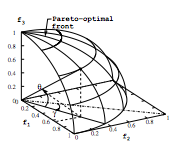
\includegraphics{img/dtlz2_pareto.png}
		\caption{Pareto Frontier of DTLZ2}
		\label{fig:problem}
	\end{figure}
	
	\begin{figure*}[htbp]
	\centering
	\begin{minipage}{0.25\linewidth}
		{\footnotesize \begin{tabular}{lr}
			\hline
			\rowcolor[gray]{.9} Setting & Value \\ \hline
			Population Size               & 100   \\
			Number of Generations         & 100   \\
			Mutation Rate                 & 0.75  \\ 
			Crossover Probability         & 0.3  \\ \hline
		\end{tabular}}
		\caption{Settings for DE}
		\label{fig:de_settings}
		\vspace{0.25cm}
		{\footnotesize \begin{tabular}{lr}
			\hline
			\rowcolor[gray]{.9} Setting & Value \\ \hline
			Population Size               & 100   \\
			Number of Generations         & 100   \\
			Domination Factor             & 0.15  \\ \hline 
		\end{tabular}}
		\caption{Settings for GALE}
		\label{fig:gale_settings}
	\end{minipage}
	\begin{minipage}{0.66\linewidth}
	\centering
		{\footnotesize \begin{tabular}{>{\tc}m{0.81in} >{\tc}m{0.75in} >{\tc}m{0.8in} >{\tc}m{0.62in}}
			\hline
			\rowcolor[gray]{.9}Algorithm & Runtime(secs) & Convergence & Diversity \\ \hline
			DE(Serial) & \stack{0.45}{0.49}{0.81} & \stack{1.80e-5}{2.23e-5}{2.56e-5} & \stack{0.37}{0.44}{0.54} \\ \hline 
			DE(Parallel) & \stack{0.28}{0.30}{0.31} & \stack{1.80e-5}{2.25e-5}{2.58e-5} & \stack{0.38}{0.43}{0.49} \\ \hline 
			GALE(Serial) & \stack{39.30}{42.05}{43.35} & \stack{5.28e-4}{5.49e-4}{5.73e-4} & \stack{0.36}{0.41}{0.49} \\ \hline 
			GALE(Parallel) & \stack{17.13}{19.11}{20.45} & \stack{5.273-4}{5.54e-4}{5.78e-4} & \stack{0.39}{0.42}{0.51} \\ \hline 
		\end{tabular}}
		\caption{Range of Results for optimizers}
		\label{fig:results_table}
    \end{minipage}
	\end{figure*}
	\section{Experiments}
	\label{experiments}
	Python is our choice of programming language. This is due to its support for efficient computation frameworks like numpy~\cite{numpy} and scipy~\cite{scipy} that enables quick prototyping and benchmarking.
	For parallelization,  we used the OpenMPI implementation of the Message Passing Interface over a python wrapper. The Open MPI Project~\cite{openMPITool} is an open source Message Passing Interface implementation that is developed and maintained by a consortium of academic, research, and industry partners.The parallelized version of the algorithm could be deployed on HPC to measure the efficiency of the algorithm. The \textit{henry2}~\cite{ncsuHPC} shared memory linux cluster by NCSU may be used for this purpose. These nodes provide up to 16 shared memory processor cores and up to 128GB of memory accessible through a dedicated queue. 
	
	For our experiments, we used 4 cores using 128 GB of shared memory
	
	\subsection{Optimization Problem}
	\label{problem}
	
	Multi-objective Evolutionary Algorithms(MOEA) require scalable test problems that help test its efficiency. Our chosen test problem is a mathematical test problem \textbf{DTLZ2} \cite{debMOEA02}, which was formulated by \textit{Kalyanmoy \textbf{D}eb}, \textit{Lothar \textbf{T}hiele}, \textit{Marco \textbf{L}aumans} and \textit{Eckhart \textbf{Z}itzler}. 
	
	\textbf{Decisions} : DTLZ2 has 30 decisions between 0 and 1.
	\[0 \leq {x}_{i} \leq 1 \ \ \ \ where \ \  i = 1,2 ,3 .... 30\]
	
	\textbf{Objectives} : Although DTLZ2 allows as to generate upto n-1 objectives where n is the number of decisions, we choose to limit the number of objectives to 3 since we can model the objectives better to visualize the pareto frontier. Limiting the number of objectives also controls the domination pressure. All the three objectives needs to be minimized. The objectives are defined as follows:
	\[{f}_{1}(x) = (1+g({x}_{M}))\cos({x}_{1} \pi/2)....\cos({x}_{M-1} \pi/2)\]
	\[{f}_{2}(x) = (1+g({x}_{M}))\cos({x}_{1} \pi/2)....\cos({x}_{M-1} \pi/2)\]
	\[{f}_{3}(x) = (1+g({x}_{M}))\sin({x}_{1} \pi/2)\]
	\[where \ \ \ \ g({x}_{M}) = \sum_{x \in {x}_{M}} (x_i - 0.5)^2 \]
	
	\textbf{Optimal Solutions} : The pareto optimal solutions corresponds to the decisions \(x_i = 0.5\) and all objective function values must satisfy \(\sum_{m=1}^M (f_m)^2 = 1\). Figure \ref{fig:problem} shows the pareto frontier that represents the optimal solutions of DTLZ2.
	
	\subsection{Measures}
	\label{measures}
	Figure \ref{fig:measure} highlights the performance evaluation measures we use to evaluate the algorithms.
	
	
	\begin{figure}[t]
		\begin{tabular}{ll}
			\hline
			\rowcolor[HTML]{EFEFEF} 
			\multicolumn{1}{l}{\cellcolor[HTML]{EFEFEF}{\bf Measure}} & \multicolumn{1}{c}{\cellcolor[HTML]{EFEFEF}{\bf  Description}}  \\ \hline
			\rowcolor[HTML]{FFFFFF} 
			{\bf Runtime}  & \begin{tabular}[l]{@{}l@{}}Time taken for the algorithm to be gener-\\ate optimal solutions.\end{tabular}\\\hline
			\rowcolor[HTML]{FFFFFF} 
			\hline{\bf Diversity}                                           & \begin{tabular}[l]{@{}l@{}}Diversity represents the spread of the prop-\\osed solutions. Ideally the solutions should\\be well distributed across the Pareto fro-\\ntier,rather than concentrated in certain\\ regions.\end{tabular}\\ \hline
		\end{tabular}
		\caption{Performance Measures}
		\label{fig:measure}
	\end{figure}
	
	\subsection{Setup}
	
	We parallelized GALE using the "island" model\cite{gustafson2006speciating}. In the "island" approach to parallelization of genetic programming, the population for a given run is divided into semi-isolated subpopulations (called demes). Each subpopulation is assigned to a separate processor of the parallel computing system. The run begins with the one-time random creation of a separate population of individuals at each processor of the parallel computer system. This is a very rudimentary approach and we will be experimenting further using a Master Slave approach.
	
	The parameters we use for Differential Evolution and GALE are shown in \ref{fig:de_settings} and \ref{fig:gale_settings} respectively.
	
	\section{Results}
	\label{results}
	
	\begin{table*}[htbp]
    \begin{minipage}{0.98\linewidth}
        \centering
        \begin{tabular}{$l@{\hspace{6pt}} *{16}{^c@{\hspace{5pt}}}}
        \toprule
        \rowstyle{\bfseries\boldmath} Processors  & 1 & 2 & 3 & 4 & 5 & 6 & 7 & 8 & 9 & 10 & 11 & 12 & 13 & 14 & 15 & 16 \\
        \midrule
        \bfseries GALE
        & 96.38
        & 50.32
        & 34.96
        & 25.92
        & 21.46
        & 17.98
        & 14.95
        & 13.17
        & 12.35
        & 10.56
        & 10.13
        & 9.14 
        & 8.43 
        & 7.67 
        & 7.58 
        & 6.97 \\
        \bfseries DE
        & 0.97
        & 0.53
        & 0.3 
        & 0.23
        & 0.17
        & 0.15
        & 0.13
        & 0.11
        & 0.11
        & 0.08
        & 0.09
        & 0.14
        & 0.1 
        & 0.09
        & 0.07
        & 0.06 \\
        \bottomrule
        \end{tabular}
        \caption{Runtimes of GALE and DE in seconds}
        \label{tab:runtimes}
    \end{minipage}
    \end{table*}
	
	\subsection{Accuracy}
	The results for runtime, convergence and diversity are shown in \ref{fig:results_table}. Each optimizer is run over a random initial sample of the population 20 times to get the range of output values. The values in the 20 iterations are shown as bar charts representing the median and inter-quartile range of the 20 runs in \fig{results_table}.  As we can see the serialized version of DE yields the lowest convergence. The diversity for all three optimizers are in the same range.
	
	
	To provide a more comprehensive comparison, we studied the optimizers and ranked them statistically. To do this we made use of the Scott-Knott procedure recommended by Mittas \& Angelis\cite{mittas13}. This method
	sorts a list of $l$ treatments with $ls$ measurements by their median
	score. It then
	splits $l$ into sub-lists $m,n$ in order to maximize the expected value of
	differences  in the observed performances
	before and after divisions. E.g. for lists $l,m,n$ of size $ls,ms,ns$ where $l=m\cup n$:
	\[E(\Delta)=\frac{ms}{ls}abs(m.\mu - l.\mu)^2 + \frac{ns}{ls}abs(n.\mu - l.\mu)^2\]
	Scott-Knott then applies some statistical hypothesis test $H$ to check
	if $m,n$ are significantly different. If so, Scott-Knott then recurses on each division.
	
	As a example, consider the following hypothetical data collected under different treatments {\em rx}:
	
	{\scriptsize \begin{verbatim}
		rx1 = [0.34, 0.49, 0.51, 0.6]
		rx2 = [0.6,  0.7,  0.8,  0.9]
		rx3 = [0.15, 0.25, 0.4,  0.35]
		rx4=  [0.6,  0.7,  0.8,  0.9]
		rx5=  [0.1,  0.2,  0.3,  0.4]
		\end{verbatim}}
	\noindent
	After sorting and division, Scott-Knott declares:
	\bi
	\item Ranked \#1 is rx5 with median= 0.25
	\item Ranked \#1 is rx3 with median= 0.3
	\item Ranked \#2 is rx1 with median= 0.5
	\item Ranked \#3 is rx2 with median= 0.75
	\item Ranked \#3 is rx4 with median= 0.75
	\ei
	Note that Scott-Knott found  little
	difference between rx5 and rx3. Hence,
	they have the same rank, even though their medians differ.
	
	Scott-Knott is better than an 
	all-pairs hypothesis test of all methods; e.g. six treatments
	can be compared \mbox{$(6^2-6)/2=15$} ways. 
	A 95\% confidence test run for each comparison has  a very low total confidence: 
	\mbox{$0.95^{15} = 46$}\%.
	To avoid an all-pairs comparison, Scott-Knott only calls on hypothesis
	tests {\em after} it has found splits that maximize the performance differences.
	
	For this study, our hypothesis test $H$ was a
	conjunction of the A12 effect size test of  and
	non-parametric bootstrap sampling; i.e. our
	Scott-Knott divided the data if {\em both}
	bootstrapping and an effect size test agreed that
	the division was statistically significant (99\%
	confidence) and not a ``small'' effect ($A12 \ge
	0.6$).
	
	
	
	\begin{figure}[t]
		{\scriptsize \begin{tabular}{l@{~~~}l@{~~~}l@{~~~}l@{~~~}c}
			\arrayrulecolor{darkgray}
			\hline
			\rowcolor[gray]{.9}  Rank & Optimizer & Median & IQR & 
			%min= 20, max= 117
			\bigstrut\\ \hline
			1 &      DE(Parallel) &    2.30$\times10^{-5}$  &  2.74$\times10^{-6}$ & \quart{1}{1}{1}{100} \bigstrut\\
			1 &      DE(Serial) &    2.36$\times10^{-5}$  &  3.04$\times10^{-6}$ & \quart{1}{1}{1}{100} \bigstrut\\
			\hline
			
			2 &      GALE(Serial) &    5.49$\times10^{-4}$  &  8.72$\times10^{-6}$ & \quart{70}{1}{71}{100} \bigstrut\\
			2 &       GALE(Parallel) &    5.54$\times10^{-4}$  &  2.21$\times10^{-5}$ & \quart{70}{10}{76}{100} \bigstrut\\ \hline
			
		\end{tabular}}
		\caption{Convergence of Optimizers. }\label{fig:convergence}
		\vspace{0.25cm}
		{\scriptsize \begin{tabular}{llllcc}
			\arrayrulecolor{darkgray}
			\hline 
			\rowcolor[gray]{.9}  Rank & Optimizer & Median & IQR & & 
			%min= 20, max= 117
			\bigstrut\\ \hline
			1 &      GALE(Parallel) &    0.416  &  0.070 & \quart{45}{6}{47}{100} & \bigstrut\\ 
			1 &      DE(Parallel) &    0.417  &  0.049 & \quart{45}{4}{47}{100} & \bigstrut\\ 
			1 &      DE(Serial) &    0.431  &  0.056 & \quart{46}{5}{48}{100} & \bigstrut\\
			1 &      GALE(Serial) &    0.432  &  0.047 & \quart{46}{4}{48}{100} &\bigstrut\\ \hline
			
		\end{tabular}}
		\caption{Diversity of Optimizers. }\label{fig:diversity}
	\end{figure}
			
	We have estimated the Scott-Knott rankings for convergence and diversity for all three of the optimizer methods. We did not estimate it for runtime since DE was almost 50 times faster than GALE, hence there was no statistical significance to measure it.
	
	From figure \ref{fig:convergence} we can see that the serialized version of DE produces the best result with rank 1, but there is no statistical difference between the serialized and parallel version of GALE in terms of convergence. The black dot in the last column shows the median value of convergence over 20 runs and the line shows the set of values between the 25th and 75th percentile. We can see that the variance for convergence is very small for all the optimizers, since the inter-quartile distance between the 25th and 75th quartile is almost 0.
	
	The figure \ref{fig:diversity} shows that there is no statistical difference in diversity between all the three methods.
	
	\subsection{Runtimes}
	
	HPC supports upto 16 processors with 128GB of shared memory. The runtimes for DE and GALE when deployed on 1 to 16 processors is tabulated in table \ref{tab:runtimes}. The results show that after 8 processors the runtime for DE starts to become constant and for GALE, the results does not stabilize. This might be because the runtimes for GALE is two orders of magnitude more than that of DE and hence the communication overhead might not be significant in its case.
	
	Based on the data in table \ref{tab:runtimes}, speed up for on different processors is illustrated in \ref{fig:speedups}. Speed up is calculated as
	
	\[SpeedUp = \frac{{T}_{Serial}}{{T}_{Parallel}} \]
	
	where ${T}_{Serial}$ is the time taken to run the optimizer on a single processor and ${T}_{n}$ is the time taken to run the optimizer parallely on \textbf{n} number of processors where n varies from 2 to 16.
	
	
	\begin{figure}[h]
		\begin{mdframed}
			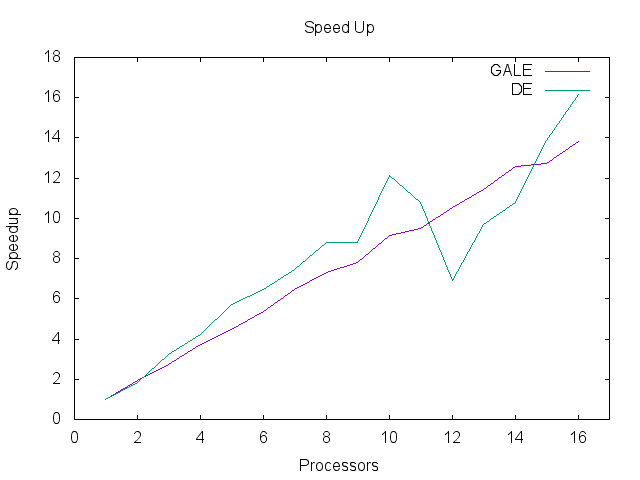
\includegraphics[width=\linewidth]{img/speedups}
		\end{mdframed}
		\caption{Speed Ups for GALE and DE}	
		\label{fig:speedups}
	\end{figure}
	
% 	\begin{figure}[h]
% 		\begin{mdframed}
% 			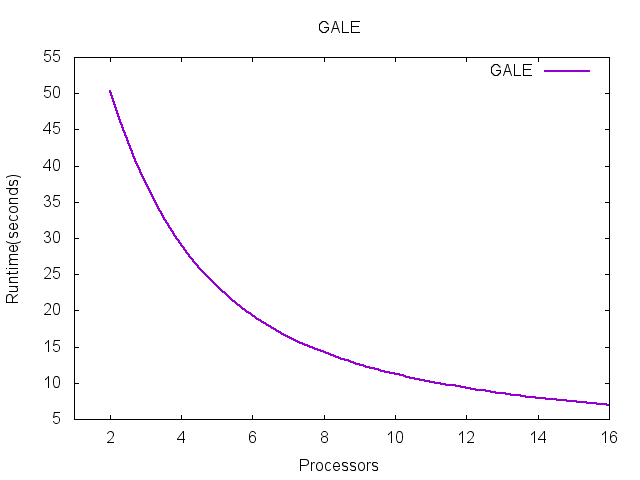
\includegraphics[width=\linewidth]{img/gale_processors}
% 		\end{mdframed}
% 		\caption{GALE: Runtime vs Processors}	
% 		\label{fig:gale_runtime}
% 	\end{figure}
	
	\section{Future Work}
	\label{future}
	
	Now that we have implemented the serialized version of the algorithms and a parallelized version of GALE, we plan to:
	\begin{enumerate}
		\item Experiment different parallelization strategies for GALE
		\item Check the scalability of the optimizer on a larger model like XOMO\cite{menzies05xomo}
	\end{enumerate}
	\bibliographystyle{plain}
	\bibliography{refs}
\end{document}